\begin{frame}{La blockchain}
    \begin{figure}
        \centering
        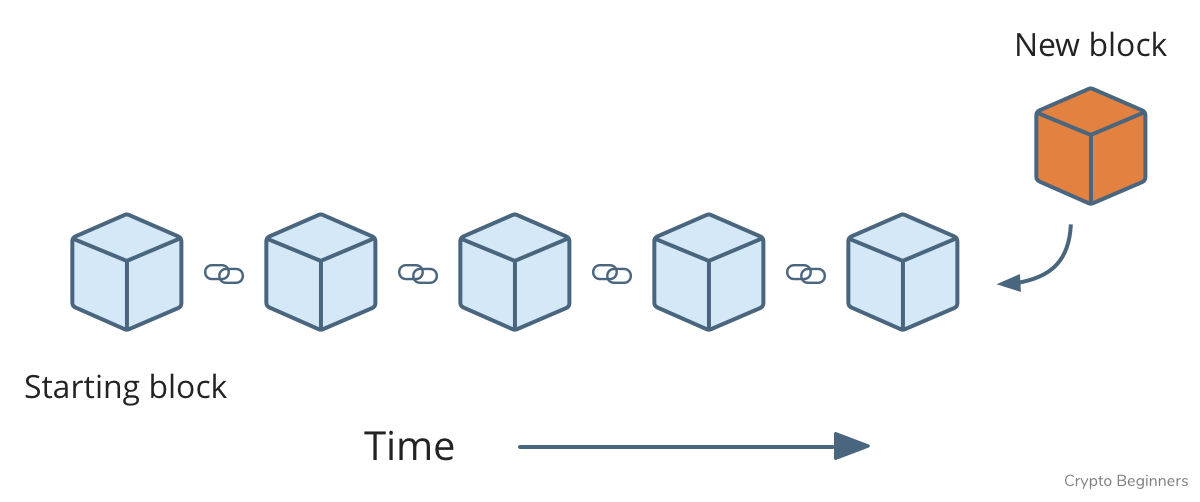
\includegraphics[scale = 0.2]{introduction/blockchain.png}
    \end{figure}
\end{frame}

\begin{frame}{Un réseau de noeud}
    \begin{figure}
        \centering
        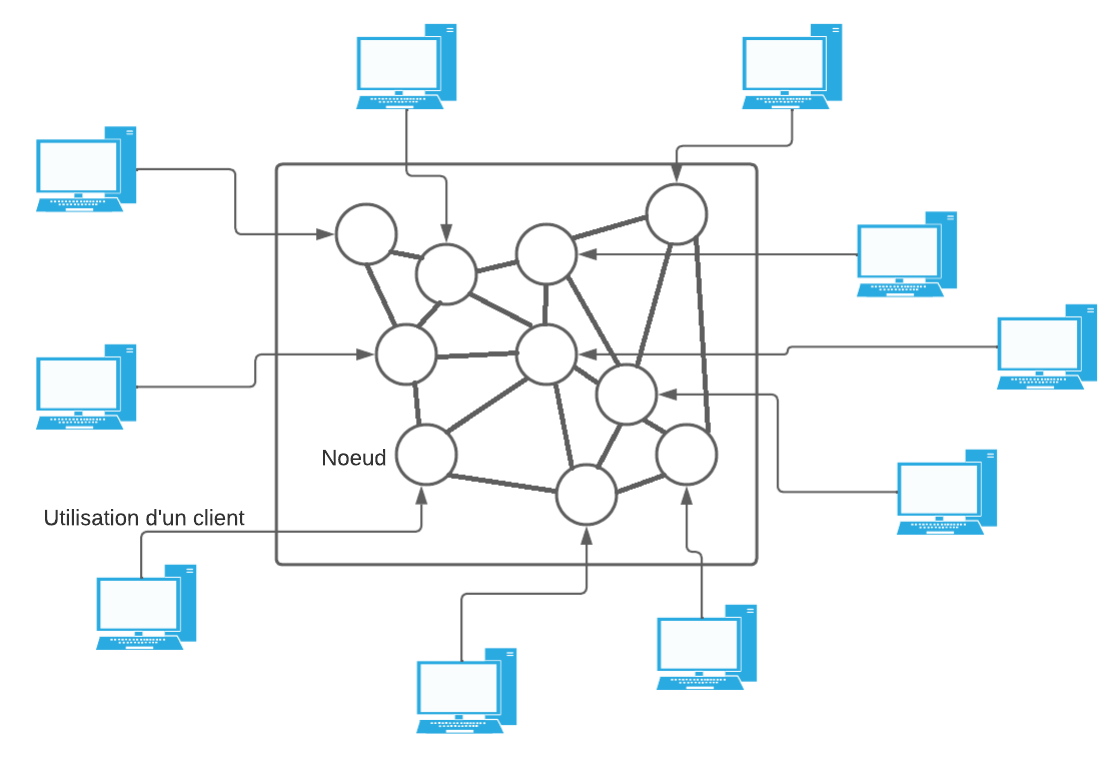
\includegraphics[scale = 0.6]{introduction/ReseauNoeuds.png}
    \end{figure}
\end{frame}

\begin{frame}{Spécificités d'une blockchain}
    \begin{itemize}
        \item Aucune autorité centrale.
        \item Abscence de hiérarchie.
        \item Immuable.
        \item Aucune présence d'informations contradictoires.
        \item Notion de partage et consensus. 
    \end{itemize}
\end{frame}

\begin{frame}{Réponse à un besoin}
        \begin{itemize}
        \item Bitcoin première cryptomonnaie avec 40,5\% du marché.
        \item Ether (Ethereum) en deuxième place avec 19,5\%.
        \item 40\% restants composés de centaines de cryptomonnaies.
    \end{itemize}
\end{frame}

    \begin{frame}{Centralisation et Décentralisation}
        \begin{figure}
            \centering
            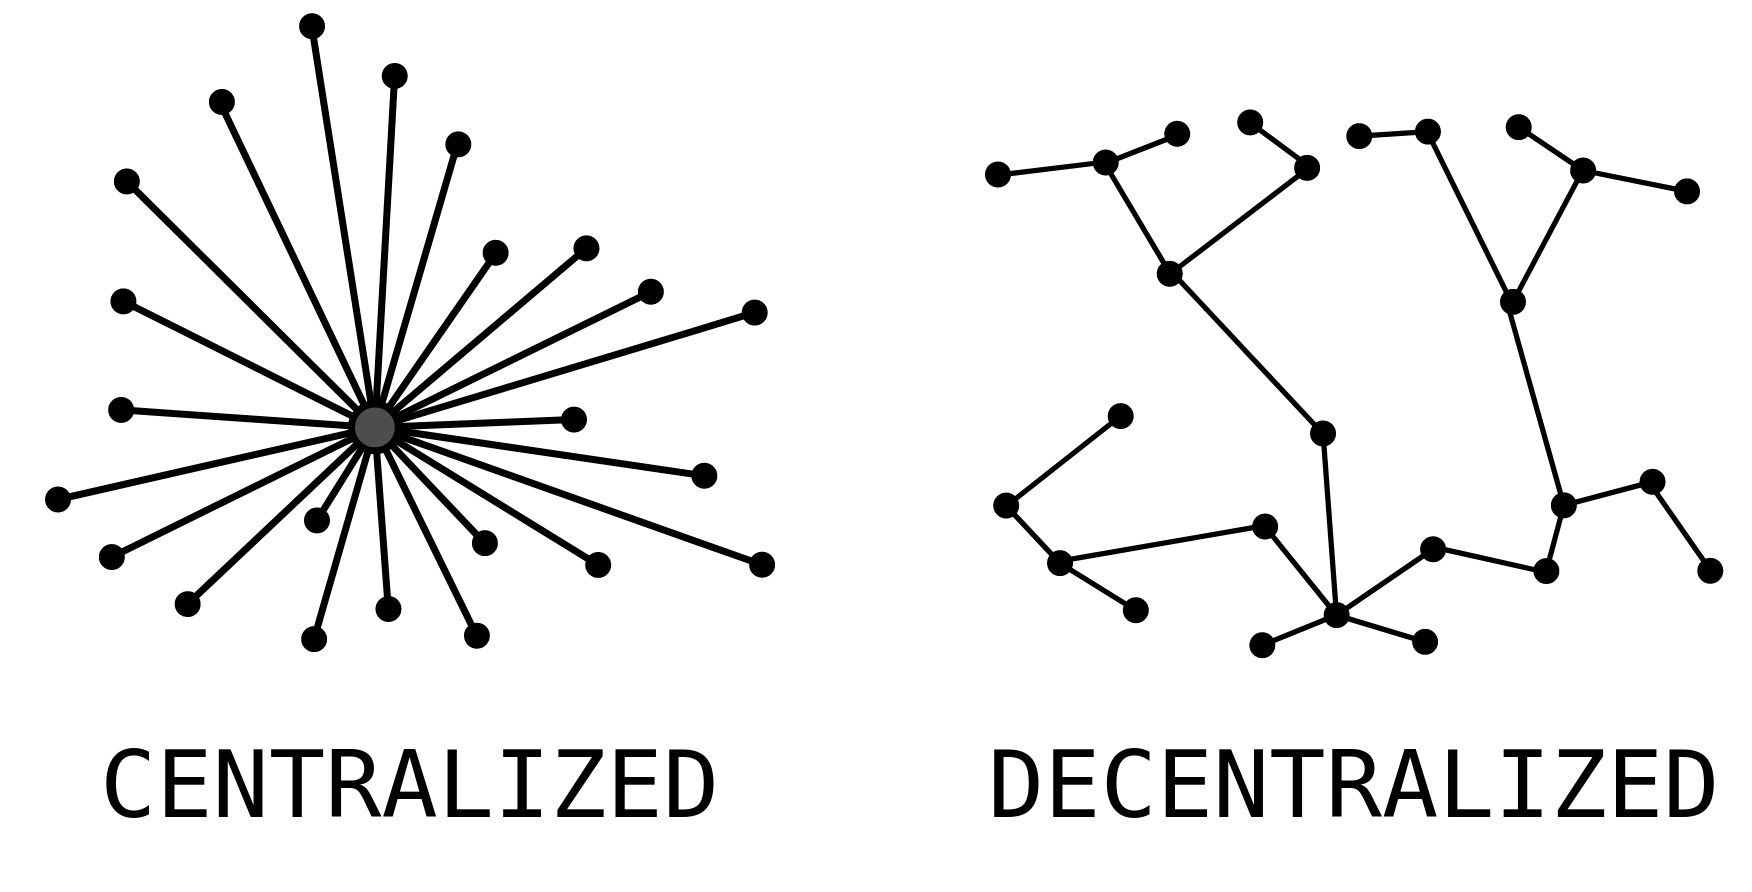
\includegraphics[scale = 0.2]{introduction/CentralDecentral.png}
        \end{figure}
    \end{frame}